\section{Compilation process}\label{section:compilation}
Compilers\index{compiler} pursue programming languages since the time languages arised. Modern compilers are often written in quite high level programming languages. Compiler of Scheme\index{Scheme} can be (and for learning purposes is) written in Scheme itself. Smart people see here typical instance of \enquote{the chicker or the egg} problem. What if we have just invented new programming language and we need to program its compiler? We need to use another programming language to program its very first compiler.

Same problem was faced by developers in the times of programming antiquity. Perfect example is the C\index{C} compiler. When C was invented, there was (naturally) no compiler for it. It had to be programmed from scratch using another programming language. Assembly\index{assembly} language was chosen. That led to quite high code complexity and very huge effort by the programmers had to be spent, so that compiler could be finished.

\subsection{Compilers, linkers, assemblers, \ldots}
Compiler is generally a converter. It does certain kind of conversion. If we talk about programming language compiler, then we naturally expect to convert textual \textit{source code} into executable\index{executable file} form. Output of compiler (of object-oriented language) is sometimes called \textit{object code}\index{object code}. Transformaton from source code\index{source code} into object code is not straigtworward and needs to be done in several steps in majority of \cpp compilers.

In fact, compiler doesn't do source code to object code transformation. It does transformation from source code to \textit{assembly language}\index{assemebly language}. Assembly language is then assembled into object code by \textit{assembler}\index{assembler}.

Object code itself can be directly executable but, in most cases, it is not. \cpp offers many functions and features via embedded standard library\index{standard library}. All functions are placed is separate dynamic-link library{dynamic-link library}. Object code contains just signatures of used functions, function bodies are stored in library and object code needs to be told where library is located, so that called standard library functions can find their bodies and execute successfully. Process of connecting library functions signatures in source code to library function bodies in library file is called \textit{linking}\index{linking} and tool perform such a process is called \textit{linker}\index{linker}. Linking can be divided into static and dynamic, see page \pageref{listing:linking} for more information.

\fdocabbrevdeclare{ELF}{ELF}{Executable and Linkable Format}
\fdocabbrevdeclare{PE}{PE}{Portable Executable}
\subsection{Executable files and its structure}
Final output of \cpp code compilation is executable file or library file. Structure of executable file differs from platform to platform. Linux uses \fdocabbrevref{ELF} and Windows uses \fdocabbrevref{PE}.

Both executable file formats differ in details but they follow the same idea. Executable file is divided into header and body in this idea. Header usually contains table with information about placement of linked libraries. This table is filled with actual information when exectuble file launches. Body of executable file includes object code.\footnote{Information in this paragraph is not entirely true but it's \enquote{correct enough} for our purposes.}

Let's look at compilation process of plain \cpp application and Qt-based application. There are many differences as different entities take part in the process.

\subsection{Classic C plus plus compilation process}
Experienced \cpp programmer is probably familiar with standard compilation process (\autoref{figure:classicpr}). This process consists of four main steps:
\begin{enumerate}
\item Makefile\index{makefile} generation utility generates desired kind of makefiles. This step is fairly optional and is not needed for small applications.
\item Preprocessor\index{preprocessor} examines input source code, replaces all occurrences of preprocessor definitions and expand macros to actual code. Files produced by preprocessor are ready to be processed by compiler.
\item Compiler\index{compiler} checks syntactical correctness of input \cpp code. If code is correct, then compilation goes on, otherwise procedure halts and error is displayed to the user. Compiler produces assembly code which is accepted by assembler.
\item Assembler\index{assembler} takes assembly code and produces machine code (object code) for target architecture.
\item Linker\index{linker} accepts compiled machine code as its input and produces executable file by linking machine code against needed libraries and adding necessary metadata and headers.
\end{enumerate}

\begin{figure}[ht]
\centering
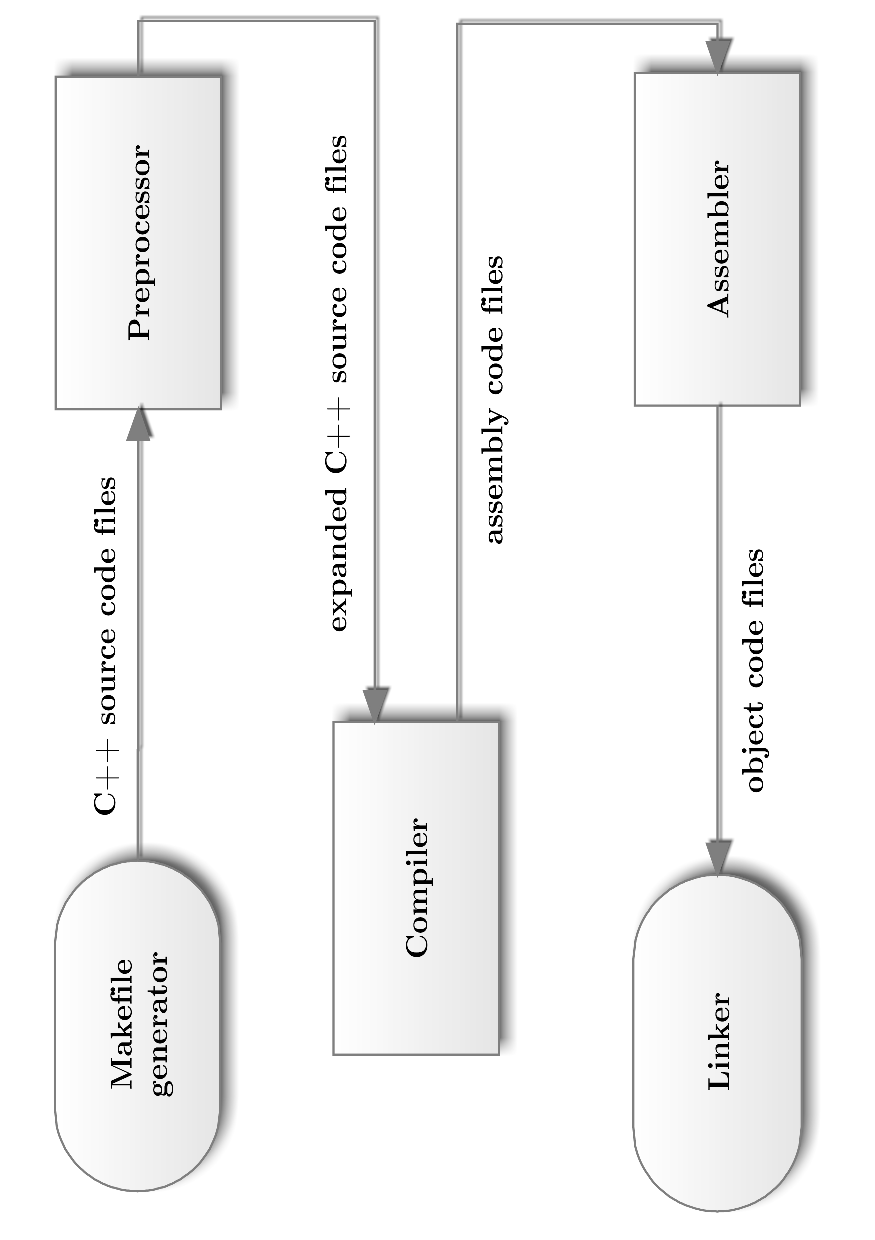
\includegraphics[angle=-90,width=11cm]{graphics/laboratory/09-classiccomp.pdf}
\caption{Classic \cpp code compilation process}\label{figure:classicpr}
\end{figure}

\fdocabbrevdeclare{moc}{moc}{Meta-Object Compiler}
\fdocabbrevdeclare{mos}{mos}{Meta-Object System}
\subsection{Qt-way C plus plus compilation process}
Qt/\cpp compilation process (\autoref{figure:qtpr} differs from classic \cpp code compilation process because \fdocabbrevref{moc}\index{\fdocabbrevref{moc}} comes into the compilation process. \fdocabbrevref{moc} one of fundamental basic stones of Qt itself. It is just more sophisticated preprocessor tool and source code generator. You will learn about \fdocabbrevref{moc} later becaus it is essential part of Qt \fdocabbrevref{mos}.

\begin{figure}[ht]
\centering
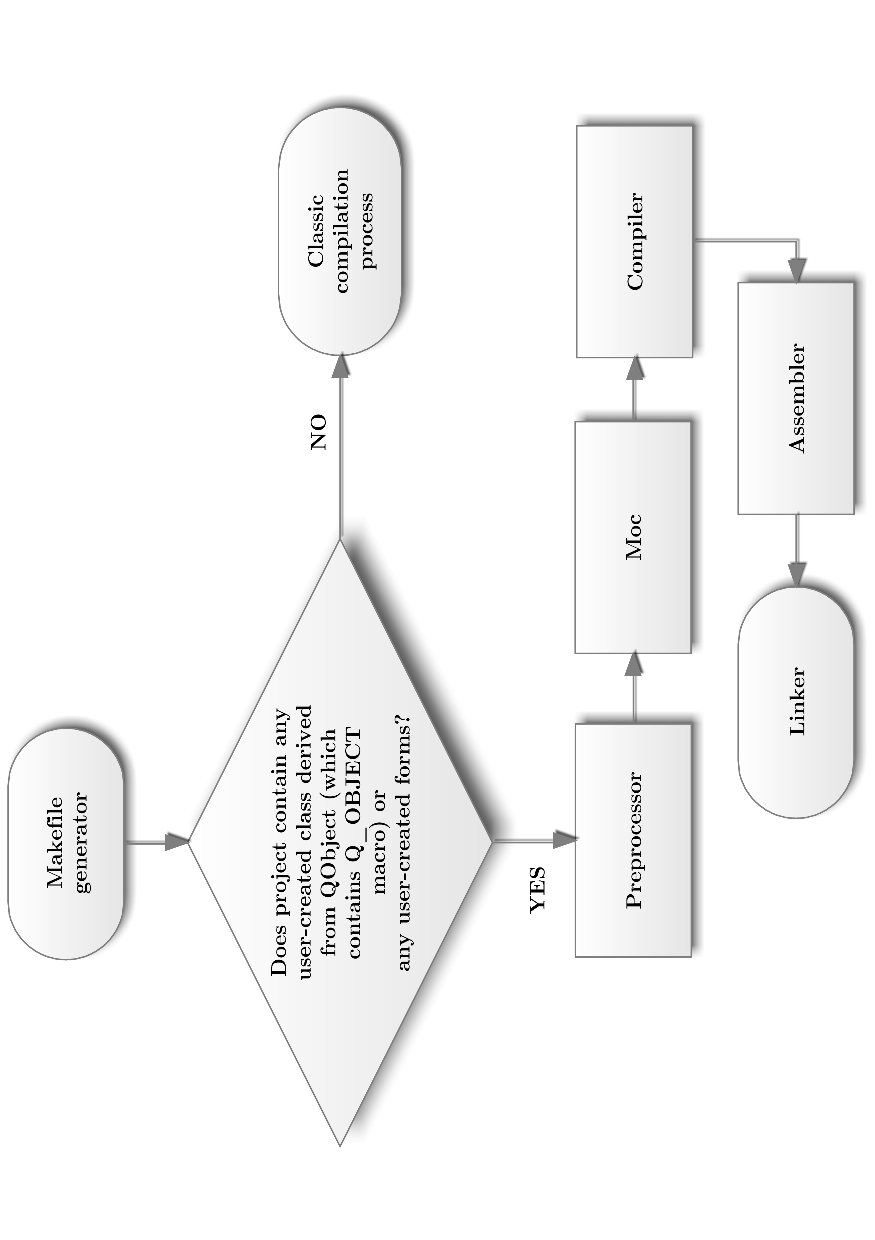
\includegraphics[angle=-90,width=14.5cm]{graphics/laboratory/10-qtcomp.pdf}
\caption{Qt-way \cpp code compilation process}\label{figure:qtpr}
\end{figure}
